%!TEX root = /Users/Nikolaj/Developer/GPU-Project/Report/Report.tex

Now that it has been established that the solution produces satisfactory results it is time to examine the increase in speed the solution provides. Four different performance test was performed each one providing a different insight into how this solution was improved compared to original C\#. The graphs depicted in this section are all from the Gpulab06 machine but full performance tests for all machines can be found in (INDSÆT APPENDIX). \\

TODO: Husk at nævne at middle stepsize er altid 2 i alle test

\subsection{Variable $x$}
While changing the $x$ values should only change the runtime with a factor, it is important to show that our solution is fast no matter what values are chosen. Changing $g$ and $r$ will have no performance effect and is therefore not included in the tests.

TODO: Graph with runtime and variable g,r,x and constant stepsize. \\
TODO: kommenter på grafen

\subsection{Variable Stepsize}
One of the advantages of using a Runge Kutta 4th order solver is that an appropiate stepsize can be chosen beforehand, enabling users to get the precision they desire at the cost of runtime. While increasing the stepsize will increase the runtime in our solution the increase is quite small compared to the increase found in both the C and C\# solutions.

\begin{figure}
\begin{center}
	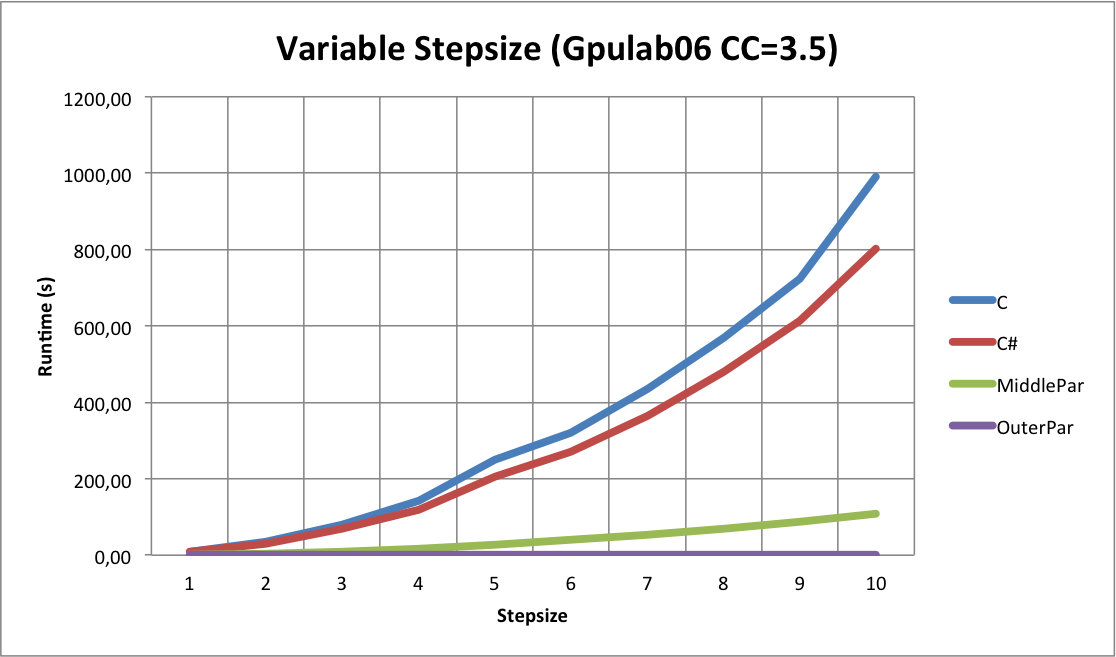
\includegraphics[width=\textwidth]{img/Gpulab-stepsize.png}
\end{center}
\caption{The impact of changing the stepsize on the Gpulab06 machine}
\end{figure}

Increasing the stepsize does increase the runtime as expected but our OuterPar solution is superior in every test we performed on all the machines. The results showed up to 550 times faster runtimes compared to the original C\# implementation.

\subsection{Variable Threads per Block}
Since the number of threads per block is set at compile time in the CUDA solution it is interesting to test what impact different amounts have on the performance.

\begin{figure}
\begin{center}
	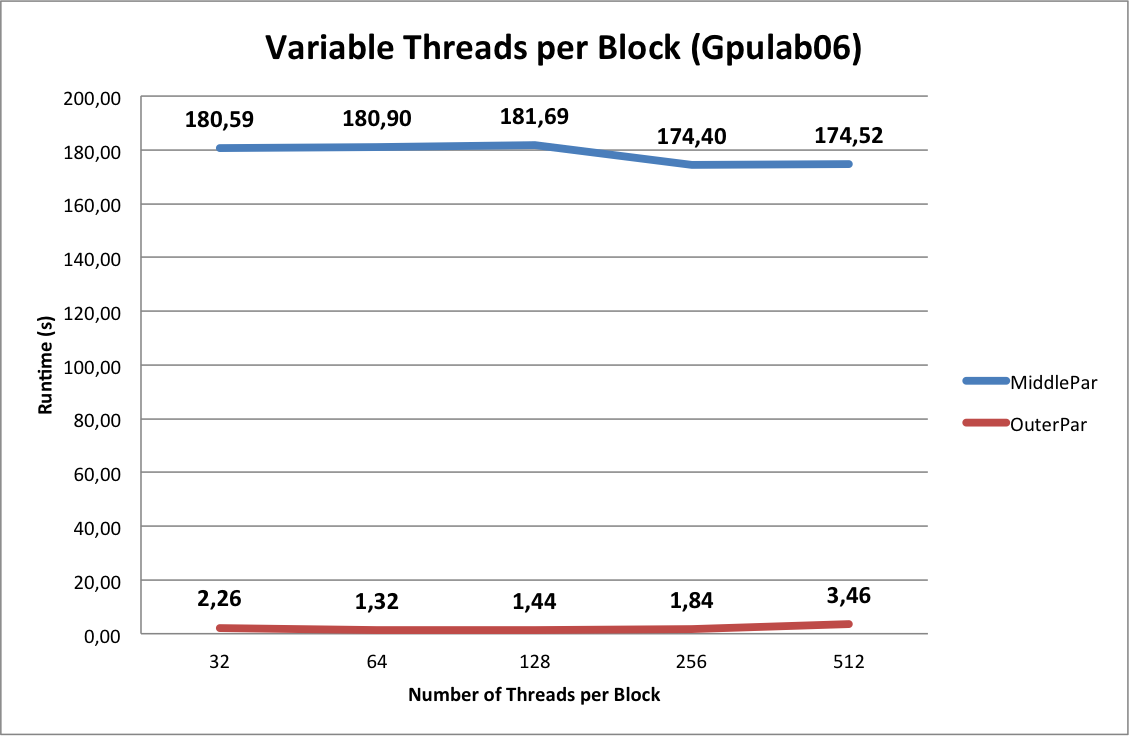
\includegraphics[width=\textwidth]{img/Gpulab-tpb.png}
\end{center}
\caption{The impact of changing the threads per block on the Gpulab06 machine}
\end{figure}
TODO: konkluder på grafen \\

TODO:
Afrunding på hele B\&C (også afvigelser i middlepar på NSJ)
